\chapter{Кирилловская стоянка}

«Готов ли ты писать главу о Кирилловской стоянке?» – спросил я себя и отправился на кухню. Там размораживалась вишня. Ею нас изредка снабжают соседи, с дачи привозят. Это какая-то удивительно сладкая вишня, но с виду самая обыкновенная. Я не дожидаюсь, пока она размерзнется полностью, и ем чуть ли не в полуледяном состоянии. Ибо вкусно.
   
Поедая такую где-нибудь на природе, я бы наверное плевал косточки на землю. Чтобы вишня тут выросла. А часть косточек не прорастет, и через много веков их откопают археологи. Они конечно же удивятся – как тут появились косточки? Ведь следы вишневой древесины рядом не найдены. Значит, косточки принесло разумное существо. Может быть несколько – стая птиц, и у каждой по вишневой косточке в клюве. Или человек с газетным кулечком, полном вишен. Но это всё будут домыслы, потому что по россыпи косточек невозможно точно восстановить, кто их сюда принес и зачем. Ведь моих-то костей тут не будет!

Другое дело, если человек ел вишню в пустынном месте, подавился, умер, был забыт, и после археологи сопоставят скелет с косточкой и сделают однозначный вывод.

Кирилловская стоянка читателю обычно представляется предметом известным, но отдаленным, как египетские пирамиды. Сжатые популярные знания таковы – в конце 19 столетия, археолог Викентий Хвойка нашел «стоянку» каменного века, возрастом 35-10 тысячелетий до нашей эры. Кости мамонта, много. И шерстистого носорога. И очаги. И кремневые орудия. Два слоя, один глубже и древнее, другой чуть современнее, а наверху горы – еще один, уже с керамикой, но еще без металла. Об этом третьем слое пишут мало, всё больше о первых двух, да рисуют картинки – дикие люди живут в шатрах, где каркас из костей и бивней мамонта шкурами обтянут. Классическая иллюстрация.

А Кирилловская стоянка ведь совсем близко, за автобазой на Богуславском спуске\footnote{На 2016 год, это база Специализированного управления механизации и автотранспорта КП «СУППР», Богуславский спуск 1, 5, 9.}. До сих пор. И не всё так просто и ясно с жильем «стоянки» – вероятно, в нижних двух слоях вообще никто не жил в прямом смысле слова. Тем более в сказочных домиках из бивней. Чтобы вести разговор дальше, я должен, как в случае с участком от Нижнеюрковской до Иорданского переулка, дать описание местности.

От Иорданского переулка надо совсем немного пройти дальше по Кирилловской, дабы попасть на Богуславский спуск, южную его часть, что отходит на юго-запад, а потом резко сворачивает на северо-запад. К югу от спуска лежат холмы и въевшаяся в них автобаза, а к северу – здания бывшего Подольского роддома, а ранее больницы Зайцева (дома 59, 61, 61-А и так далее по Кирилловской). В 2021 году там офисы компании «Фармак».

Богуславский спуск коромыслом огибает автобазу, «медицинский квартал» и бывшие объекты промзоны, обретшие вторую жизнь с 2014 года. С северо-западной стороны вход на Богуславский преграждают ворота на охраняемую территорию. В южной же части спуска проход открыт, там постоянно дежурят в машинах, отдыхая, наряды охранных патрулей, и пустынная дорога будто въезжает по террасе, сначала прямо, потом поворачивая, постоянно и плавно наращивая высоту.

Богуславский спуск впервые появляется на картах конца 19 века как Богословский переулок. Богословский понятно почему – от сгинувшего, но где-то здесь обретавшегося монастыря. Переулок был проложен перпендикулярно Кирилловской улице в овраге между нынешними отрогами с дачами «Кожевника» и тогда равным с ним по длине отрогом Кирилловской стоянки. 

Начинался переулок не там, где теперь Богуславский спуск, а по месту Подольского роддома, Кирилловской 61, где оканчивался овраг, что лежит между упомянутыми отрогами. Наверху овраг подходил к улице Подольской (не существует, соединялась с севером Половецкой, по крайней мере на 1913 год). Вдоль оврага протекал ручей, на коем вплоть до стыка 19 и 20 веков был пруд. 

В 1930-х уже Богуславский переулок имел вид дороги от улицы Куренёвской, как тогда переименовали Кирилловскую, к перекрестку Нагорной, Половецкой и Новобоговутовской (в 2021 Богуславский примыкал бы к Нагорной 27-А). Не столь прямой, как раньше. Но вплоть до конца семидесятых по нему еще можно спуститься от Лукьяновки и Татарки, а название «спуск» оправдано предназначением. А потом, кроме прочего к Олимпиаде 1980, наверху затеяли стройку гостинично-спортивного комплекса «Авангард». Так верхушка Богуславского спуска была отделена от Лукьяновки с Татаркой, а сам «спуск» как улица изогнут на север и северо-восток с тем, чтобы снова подключиться к улице Кирилловской. 

В месте первого, если считать с востока на запад, поворота Богуславского спуска, над ним нависает огромный мыс холма с дачами «Кожевника». Там у обочины, слева лежат бетонные блоки. Взобравшись мимо них можно выйти к самому склону, и если затем пойти налево, доберетесь по террасам с родниками до задворков фабрики молочной кислоты. По ходу открывается сказочный вид – наверху за край почти отвесной горы цепляются избушки, к ним снизу зигзагами проложены ступени.

Автобаза входит в горную цепь эдакой бухтой, словно раздвигая холмы. Плоское место это неспроста напоминает пустырь за кирпичным заводом Рихерта. Здесь тоже был горный отрог, почти весь срытый для нужд другого кирпичного завода – Зайцева. Именно на этом отроге и обнаружил Хвойка то, что получило имя Кирилловской стоянки. Сейчас от нее, от раскопанного мыса, уцелел кусочек за автобазой, напротив отрога с «Кожевником». Примерные координаты: 50°28'23.59"N 30°29'20.42"E.

Если же за бетонными плитами пойти направо и вперед, по дорожке между отрогом «Кожевника» слева и стеной автобазы справа, мимо возвышающейся за ней сторожки и шумящего в коллектора ручья (что течет под оврагом между «Кожевником» и огрызком мыса стоянки), то упретесь в забор дачного товарищества, с калиткой. Дорожка там поворачивает вправо и ведет к лестничкам, устроенным на уступах. Если встать к калитке лицом, то слева дальше, уже за забором идет, образуя берег оврага, мыс «Кожевника», а по правую руку, наверху, будет уцелевшая часть раскопанного Хвойкой склона, известного по знаменитому снимку.

\begin{center}
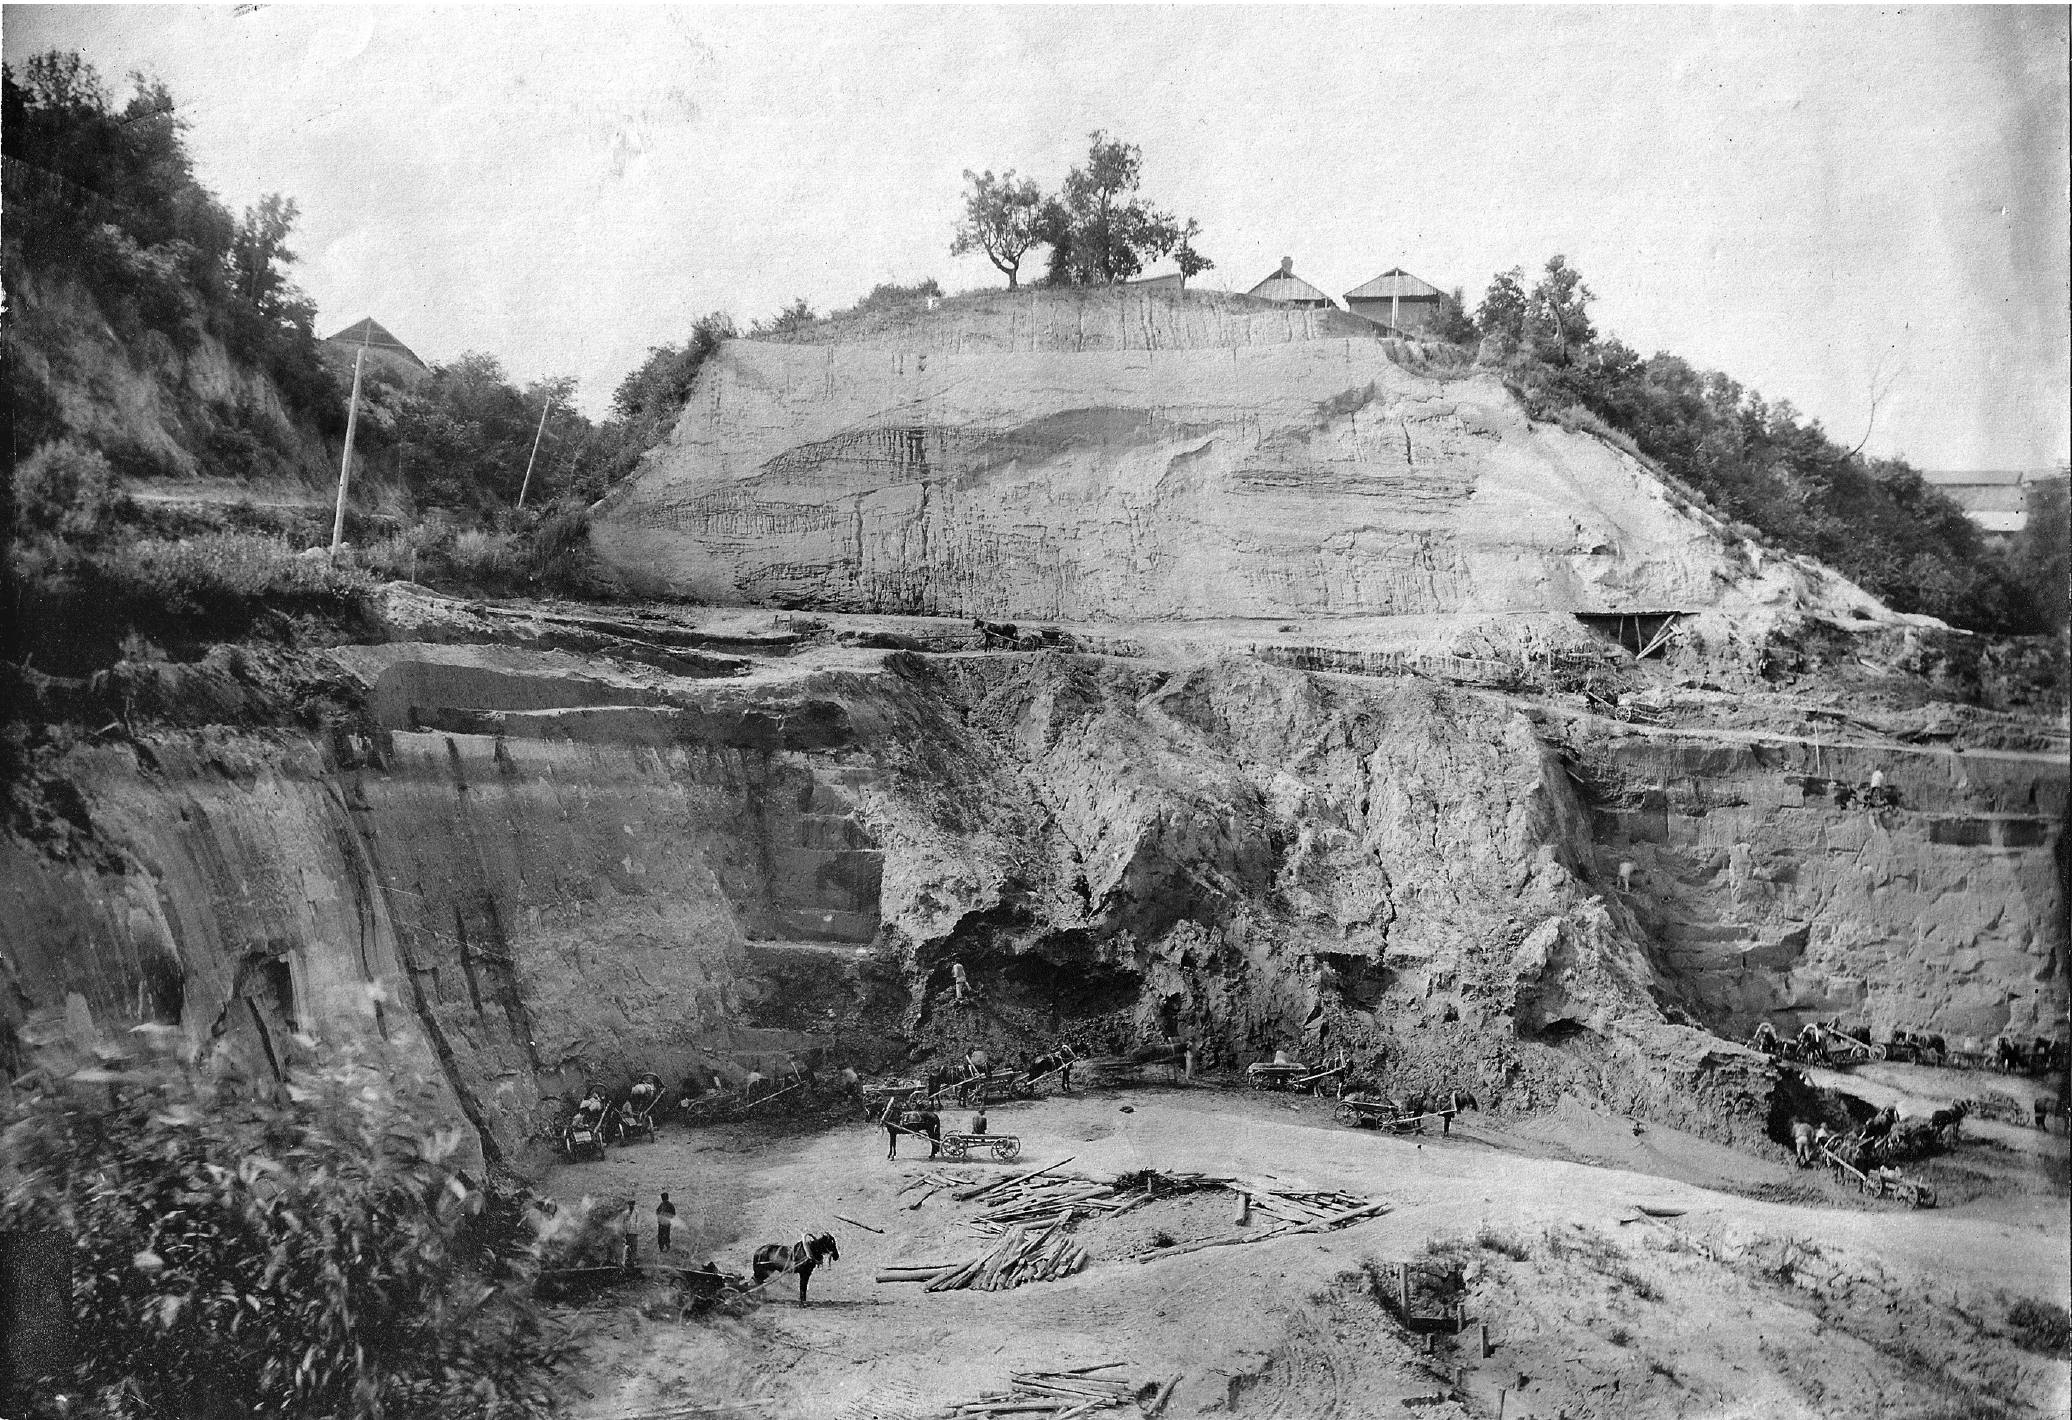
\includegraphics[width=\linewidth]{chast-kirvys/kirstoy/kirst-02.jpg}

\textit{Раскопки, фотография Хвойки, конец 19 века.}
\end{center}

\newpage

\begin{center}
\includegraphics[width=\linewidth]{chast-kirvys/kirstoy/\myimgprefix IMG_20131020_163257.jpg}

\textit{Остатки мыса раскопок, фото 2013 года.}
\end{center}

На современном снимке, верхняя часть – то, что осталось от раскопанного и уничтоженного отрога. А вот нижняя часть вызывает у меня вопросы. Это некий бугор, испещренный узкими обвалившимся лазами. Я светил туда фонариком, но видел только осыпавшиеся подземные ходы. Что это такое, трудно предположить.

От бугра можно начать лезть на склон. Самый его верх огражден забором, надо полагать, тоже дач «Кожевника», переползших и на гору по северную сторону оврага. Взбираясь под край обрыва, надо быть предельно осторожным, чтобы не навернуться. Высоко! Полное восхождение я снял и показал в фильме «Возвращение в Логово Змиево». Фотографии далее сделаны с небольшого уступчика почти наверху. На первой запечатлен открывающийся оттуда вид на автобазу. На ее месте раньше продолжался этот холм, и под ним была Кирилловская стоянка, а на его поверхности – первобытные землянки. Здания в кадре примыкают к адресу Богуславский спуск, 3.

\newpage
\vspace*{\fill}
\begin{center}
\includegraphics[width=\linewidth]{chast-kirvys/kirstoy/\myimgprefix IMG_20131020_162441.jpg}
\end{center}

\begin{center}
\includegraphics[width=\linewidth]{chast-kirvys/kirstoy/\myimgprefix IMG_20131020_162454.jpg}
\end{center}
\vspace*{\fill}
\newpage

\begin{center}
\includegraphics[width=\linewidth]{chast-kirvys/kirstoy/\myimgprefix IMG_20131020_162438.jpg}
\end{center}

Остальные две фотографии – кромка обрыва и снимок с противоположным ракурсом. Деревья тут не удерживаются, падают.

Вообще там, на самой верхотуре, два уступа, ниже и выше. Высший – правее, если смотришь на холм. Но туда сложнее залезть. Первый просто штурмуешь, а другой надо чуть обойти и потом, прижавшись к суглинной стенке, ступать по узкому, грозящему обвалиться карнизу. А он прерывается, и надо скакать. Я проделывал это, держа в одной руке видеокамеру. Бывают неотвратимые вещи, про которые понимаешь, что опасно рисковать, можно сломать шею, но ценность исследования и собственная дурость перевешивают чувство самосохранения. Я был наверху склона с Кирилловской стоянкой! Вот, могу показать на старинной фотографии место, куда долез. И что там? А вот, видео и снимки есть, пожалуйста. Впервые за сто с лишним лет. Никто тут альпинизмом не занимался, землю не рыл, сама только обваливалась.

Историческое ощущение, что я тут за век один, было фоновым. Кураж гасился насущными делами – следить, чтобы не упасть, не забыть снять всё на видео и сфотографировать. А что снимать? Что важно, что потом пригодится исследователям?

Внизу стоял на стрёме Коля. Я старался не попасть в поле зрения охранников, ибо краеведческие полевые изыскания обычно вызывают у них подозрение. Кто такие, зачем камера, фотоаппарат, что делаете? Простые люди здесь не ходят. Вы злоумышляете!

Надо было запечатлеть всё быстро и сваливать.

Вообще, как мы это место нашли. Началось с того, что я поехал на Петровку за книгами и купил пачку брошюрок про Киев, выпущенных в 1982 году издательством «Наукова думка». Среди них была книжка Дмитрия Телегина «Там, где вырос Киев». Телегин помимо прочего поведал о Кирилловской стоянке и о том, что ученые считали, будто она давно застроена. Думаю, ученые особо просто не заморачивались этим вопросом и не выходили на местность. И вот краеведы из Института Автоматики МинСвязи, что на улице Татарской, В. Черкун и Е. Малаховский, нашли 15-метровый остаток мыса, где Хвойка проводил раскопки стоянки, и провели туда Телегина, со стороны Татарки, на восток. Упомянул Телегин в книге и автобазу.

Это засело у меня в голове. Сразу отправиться на поиски не было ни времени, ни – тогда – особого желания.

Спустя некоторое время, когда мы снимали первый сезон «Киевской амплитуды», однажды договорились встретиться для съемок очередной серии. Никто кроме меня не смог приехать, и я, немного поторчав наверху станции метро Лукьяновка, решил побродить сам. Мой рюкзак был набит набором вещей, которые я таскал на вылазки – камера, фотык, фонарик налобный, фонарик ручной, газовый баллончик, еще всячина.

Тучи сгущались, я прошел до Багговутовской, свернул на славную покойницкой тишиной Пугачева, а оттуда в незаметный переулок на Врубелевский спуск, где до революции ходил трамвай. Нынешние любители старины с придыханием именуют окрестности «Киевской Швейцарией». Сейчас это хреновейшая асфальтовая дорожка, идущая вдоль гаражей над Репяховым яром. Дорожка прерывается ямами, возобновляется, затем вовсе исчезает и надо топать среди мусора и зарослей репяхов.

Пошел ливень, и единственное, что у меня не промокло, это кроссовки «Адидас». Камуфляжная куртка, штаны – всё отяжелело от воды. Я выбрался на дно яра, где проложены бетонные плиты. Поверх всё занесено глиной от ручья, частично спущенного в коллектор. Из-под крутых берегов яра сочатся родники и через непролазные дебри репейника и лопухов несут с собой глину.

Время от время делая снимки, я бодро зашагал по яру в сторону психбольницы имени Павлова. Глина образовала на дороге островки, у меня был выбор – идти по ручьям между ними, или увязать в глине. Я предпочел глину.

На повороте к Павловке почему-то скопилось много такси, я не хотел попасть под машину, и подошел к горе, на которой стоит больница. Там на склоне я раньше, по видео, заприметил вроде бы пещерку под корнями дерева. Кстати надо ее попробовать найти.

Дождь – проливной! Я цепляю фонарик на лоб, карабкаюсь, пачкаю ладони об черные стволы деревьев. Вход в пещеру или просто яма? Снизу на меня глядят люди, принимая за одного из пациентов, которых часто можно повстречать в округе. Сосредоточенно свечу фонариком в яму. Ага, это просто пустота под корневищем. Надо спускаться! Снова перехватываю деревья.

Уже все промокло, холодновато, надо домой двигать. Но черт подбивает меня исследовать Кирилловские высоты. Думаю – пройду вдоль Кирилловской, буду залезать всюду, куда получится, а затем поверну к метро. Около Смородинского спуска я открыл для себя новую тропку, частично умощенную камнем и кирпичом – и едва не полетел с нее носом вперед. Позже я узнал, что это были окрестности усадьбы художника Светославского. Я осмотрел несколько участков склона, затем обошел новые офисные здания по правую руку, да «Фармак» и, свернув на Богуславский спуск, забурился в обход, между автобазой и склоном. Тогда-то я нашел ручей в коллекторе и остатки отрога, под которым рыл Хвойка – однако не просёк, что это Кирилловская стоянка.

Дальше я упорно лез, надеясь выбраться на противоположную сторону «бухты», чтобы отыскать пещеры, связанные с делом Бейлиса, но из опасения спалиться перед охранниками пришлось медленно возвращаться, прячась за кустами и мусором. Кстати на современных электронных картах какой-то фантазер ввел для этой местности название «Богуславщина». Выдумка! Никогда такого названия не было.
 
Позже я более основательно стал собирать разрозненные и, как оказалось, довольно скудные сведения о Кирилловской стоянке. Мне на глаза попал план местности, нарисованный Хвойкой, и там был ручей вдоль горного мыса. Ага! Вот она, зацепка! Сопоставив всё по картам, аэро и спутниковым снимкам, мы с Николаем Арестовым отправились туда уже в сухую погоду, тщательно идя вдоль склонов горной гряды со стороны Иорданского кладбища – важно было вживую проверить ориентиры. И да, разрытый Хвойкой мыс оказался точно в вычисленном месте.

И вот стою под краем его вершины, надо мною ограда, я на узкой полоске глинистого уступа, негде толком развернуться. Сбоку сверху невнятно слышится музыка – там чья-то дача, живут и не ведают, где. С уступа гляжу на автобазу и вспоминаю написанное в восьмидесятых Телегиным, что построили ее недавно, а краеведы из Института Автоматики предлагали поставить на уцелевшем месте Кирилловской стоянки памятный знак. И грезил Телегин новыми раскопками... 
 
Нет ни знака, ни раскопок. Кирилловская стоянка снова погрузилась в забытие, пока мы не пришли к ней с видеокамерой.

Сложно представить, что внизу не было этих грузовиков, тракторов, хозяйственных построек, собственно и самого «низа», а вперед выдавался отрог, такой же, как находящийся рядом от него к югу, с дачами «Кожевника».

В обозримом прошлом, в 19 веке, перед отрогом, со стороны Кирилловской улицы, было две усадьбы. Юго-восточная – Багреева, северо-западная – производителя валенок Зиваля. Соответственно часть склонов отрога принадлежала Багрееву, и часть – Зивалю. По усадьбе Зиваля и вдоль южного склона, мимо ручья, проходила дорога и затем  тропа на Лукьяновку – собственно Богословский переулок. А вдоль усадьбы Багреева и по другую сторону отрога, вдоль его северного склона, шла дорога к кирпичному заводу Багреева – а точнее, купчихи Ксении Ивановне Тереховой-Багреевой.

Поглядим на карты, нарисованные Хвойкой. У меня два варианта карты отрога, сканы плохого качества, но других нет. Один, на русском языке, взят из «Трудов одиннадцатого Археологического съезда в Киеве» (1899, том 1) – статья «Каменный век среднего Приднепровья», другой, с подписями на украинском, из альманаха «Матеріали до українсько-руської етнології, Вовк Хв.» (1899, том 1). В том же альманахе дан ценнейший общий план местности, начнем с него.

\begin{center}
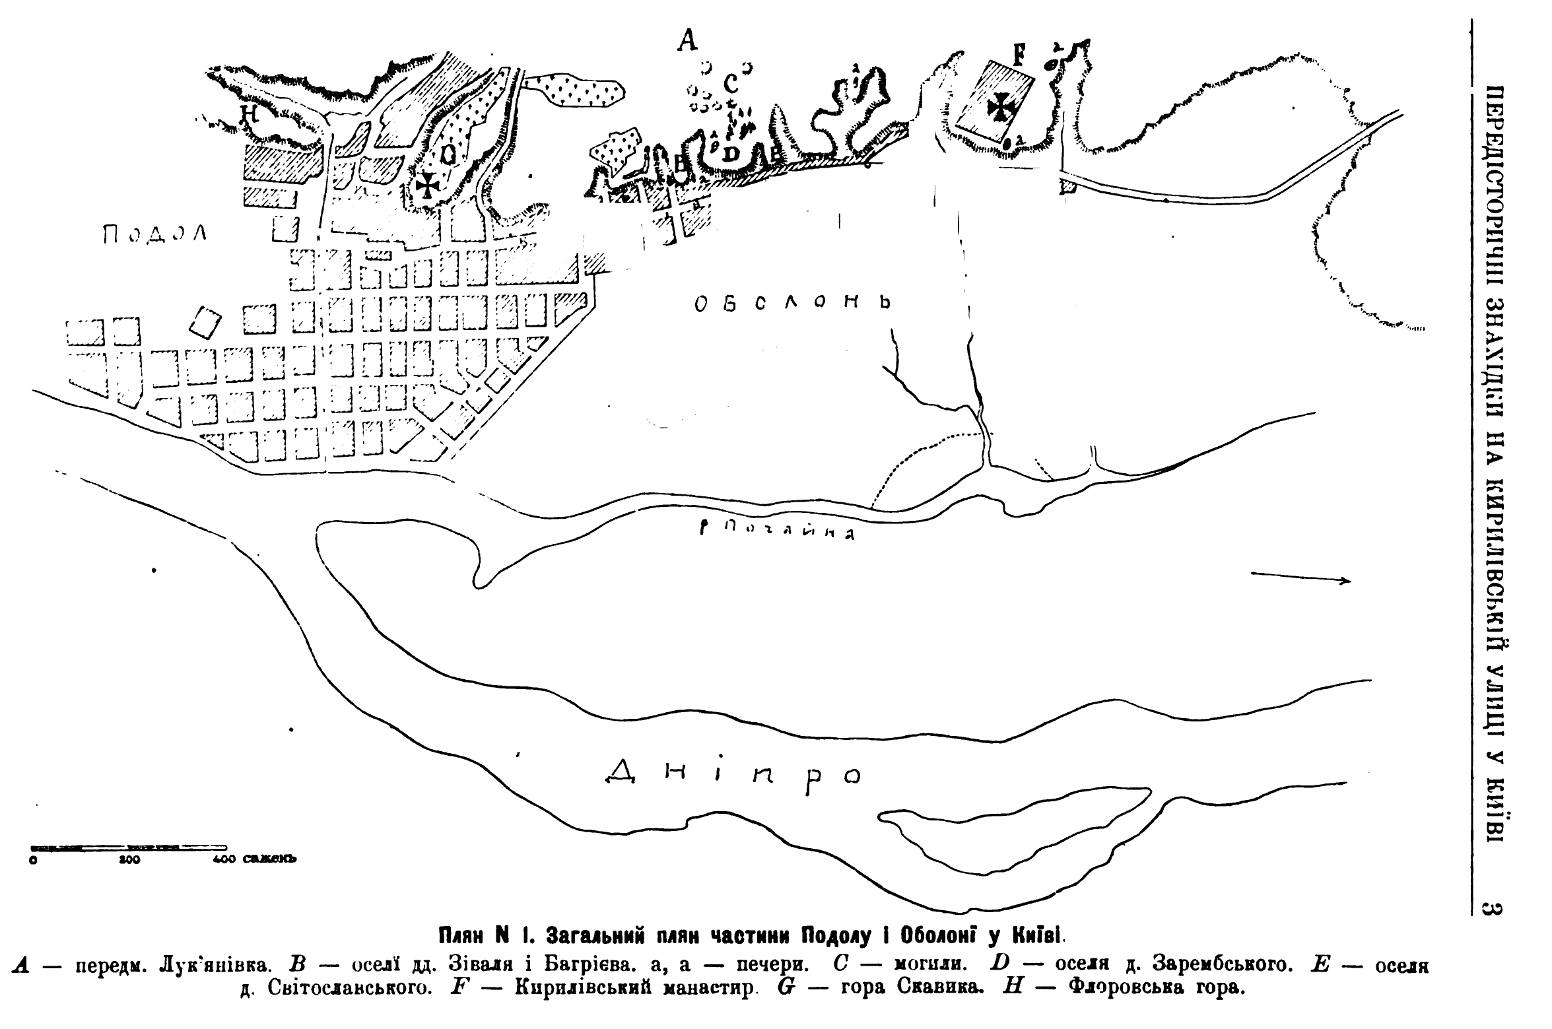
\includegraphics[width=\linewidth]{chast-kirvys/kirstoy/1893-hvoyka-main.jpg}
\end{center}

%По легенде внизу карты вы сами разберетесь, что к чему, но сделаю несколько примечаний.

Карта из альманаха Вовка, как и прочие материалы, помещенные им, получены от самого Хвойки и неких «земляков». Я пробовал наложить карту на современные и некоторые старинные, и не добился точного совмещения объектов, поэтому о многом сужу на глаз. Слева направо.

Буква «H» – Замковая гора, у Вовка Флоровская, как писал Хвойко не знаю.

Далее гора с длинным кладбищем и буквой вроде бы «C», а на деле это коряво написанное «G» – Щекавица.

Правее нее, через дорогу (Нижнеюрковская?) еще одно длинное кладбище, никак не согласующееся с известными нам местами кладбищ, и его трудно к чему-либо отнести, ибо около Щекавицы нет Рогаток. Не буду трактовать. 

Ниже этого второго кладбища еще одно, рядом с ним непонятный «бумеранг», и ниже кусочек креста – ага, Иорданская церковь. Две части кладбища на плане упрощены в одно.

Правее идет мыс с первой по счету буквой «В» – это мыс с «Кожевником». На месте «бухты» справа от этого мыса и был отрог с Кирилловской стоянкой, затем срытый до известного обрыва с фотографии.

Следующий мыс – «D» – это отрог северо-западнее от Кирилловской стоянки и нынешней автобазы (скорее всего, залезая на ее западную часть).

Выше, буквой «С» в украинском варианте карты написано «могилы», а это значит – курганы. 

Буквой «а», которая у Хвойки иногда похожа на «2», обозначены пещеры. Перечислю их слева направо.

Первая – между «B» и «D», ниже их, у начала бухты срытого отрога. В самом деле, там, по Кирилловской 59-63, где была больница Зайцева, есть сведения о какой-то древней пещере на задворках строений.

Далее группа пещер на склоне отрога, противоположном западному склону срытого отрога Кирилловской стоянки. На карте – чуть левее и выше буквы «D». По современным ориентирам речь идет о местности к западу от автобазы (и западной ее части). В одной из этих пещер обнаружили почти обескровленный труп мальчика Андрея Ющинского, жертвы в знаменитом деле Бейлиса.

Затем, как понимаю, группа пещер на нынешнем Смородинском спуске, среди них Кирилловская пещера или Змиева. Подписаны как «29», где одна цифра над другой.

Следующую «а» Хвойка поместил под Кирилловской церковью (буква «F»), у северо-западного угла церкви, на северном склоне холма. И еще одна «а», пещера, тоже около Кирилловской церкви, в сторону Кирилловской улицы.

Поглядим теперь на две карты мыса Кирилловской стоянки, по месту коего теперь автобаза на Богуславском спуске.

\begin{center}
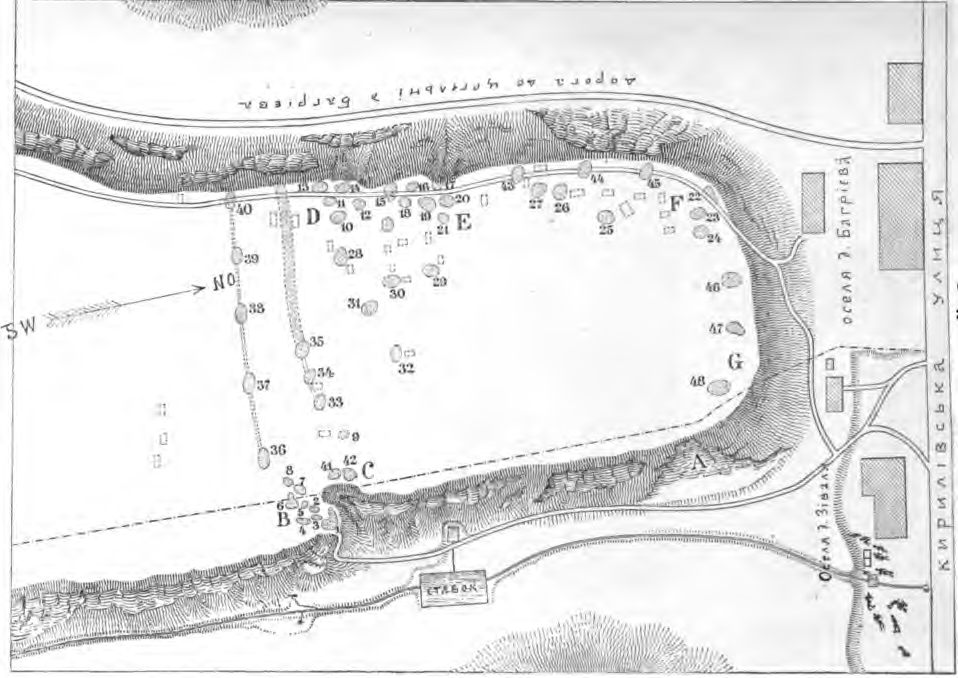
\includegraphics[width=\linewidth]{chast-kirvys/kirstoy/1893-hvoyka-01.png}
\end{center}

\begin{center}
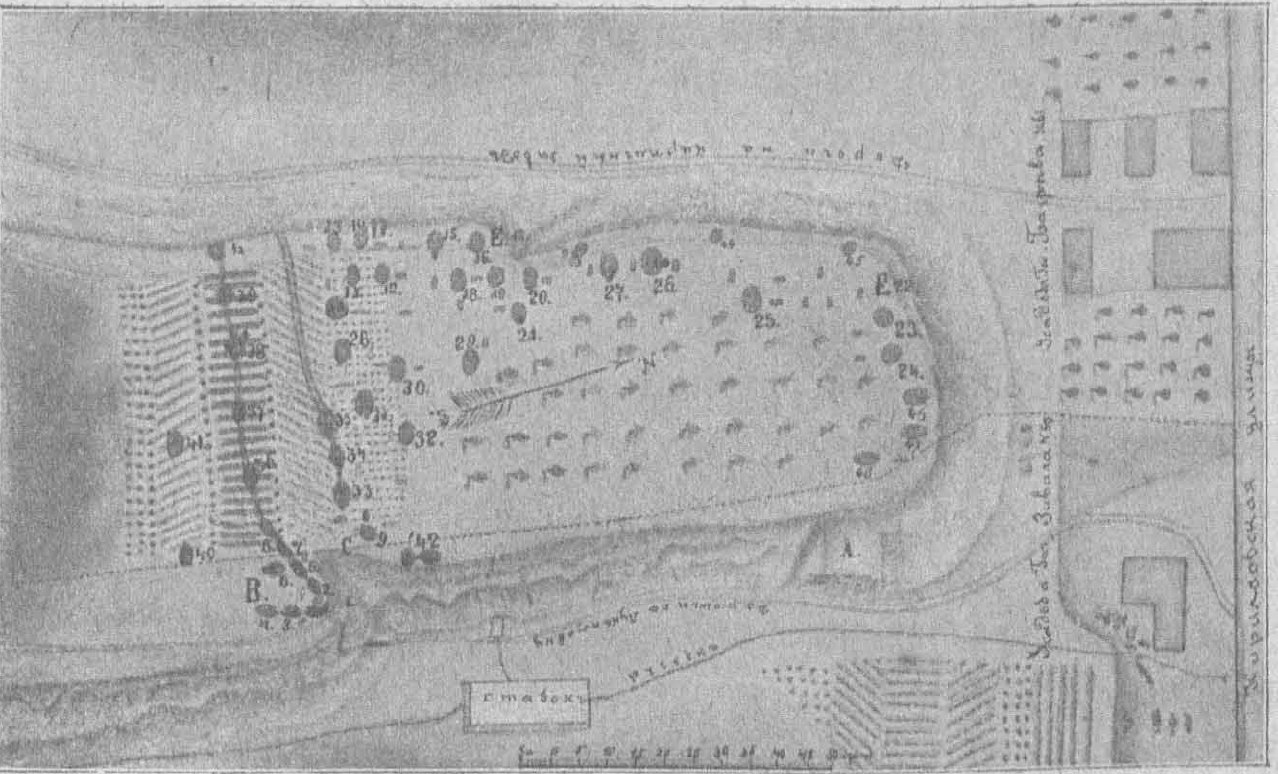
\includegraphics[width=\linewidth]{chast-kirvys/kirstoy/1893-hvoyka-02.png}
\end{center}

Они относятся к раскопкам самого верхнего культурного слоя, Хвойка связал его с неолитом. На глубине до трех метров – никаких мамонтов, а черепки керамики, кости более современных животных, обвалившиеся землянки.  

Для ориентации – внизу карты, под ставком и ручьем – отрог с дачами «Кожевника».

Номерами Хвойка пометил свои находки на плато холма и подробно описал каждую в статье «Каменный век среднего Приднепровья». Но этот почти поверхностный культурный слой Хвойка обнаружил позже древнейших, поэтому и я не стану забегать вперед.

Для пущей наглядности приведу еще кусок плана 1845 года, ориентированного как если бы мы стояли на Кирилловской улице и глядели на высоты:

\begin{center}
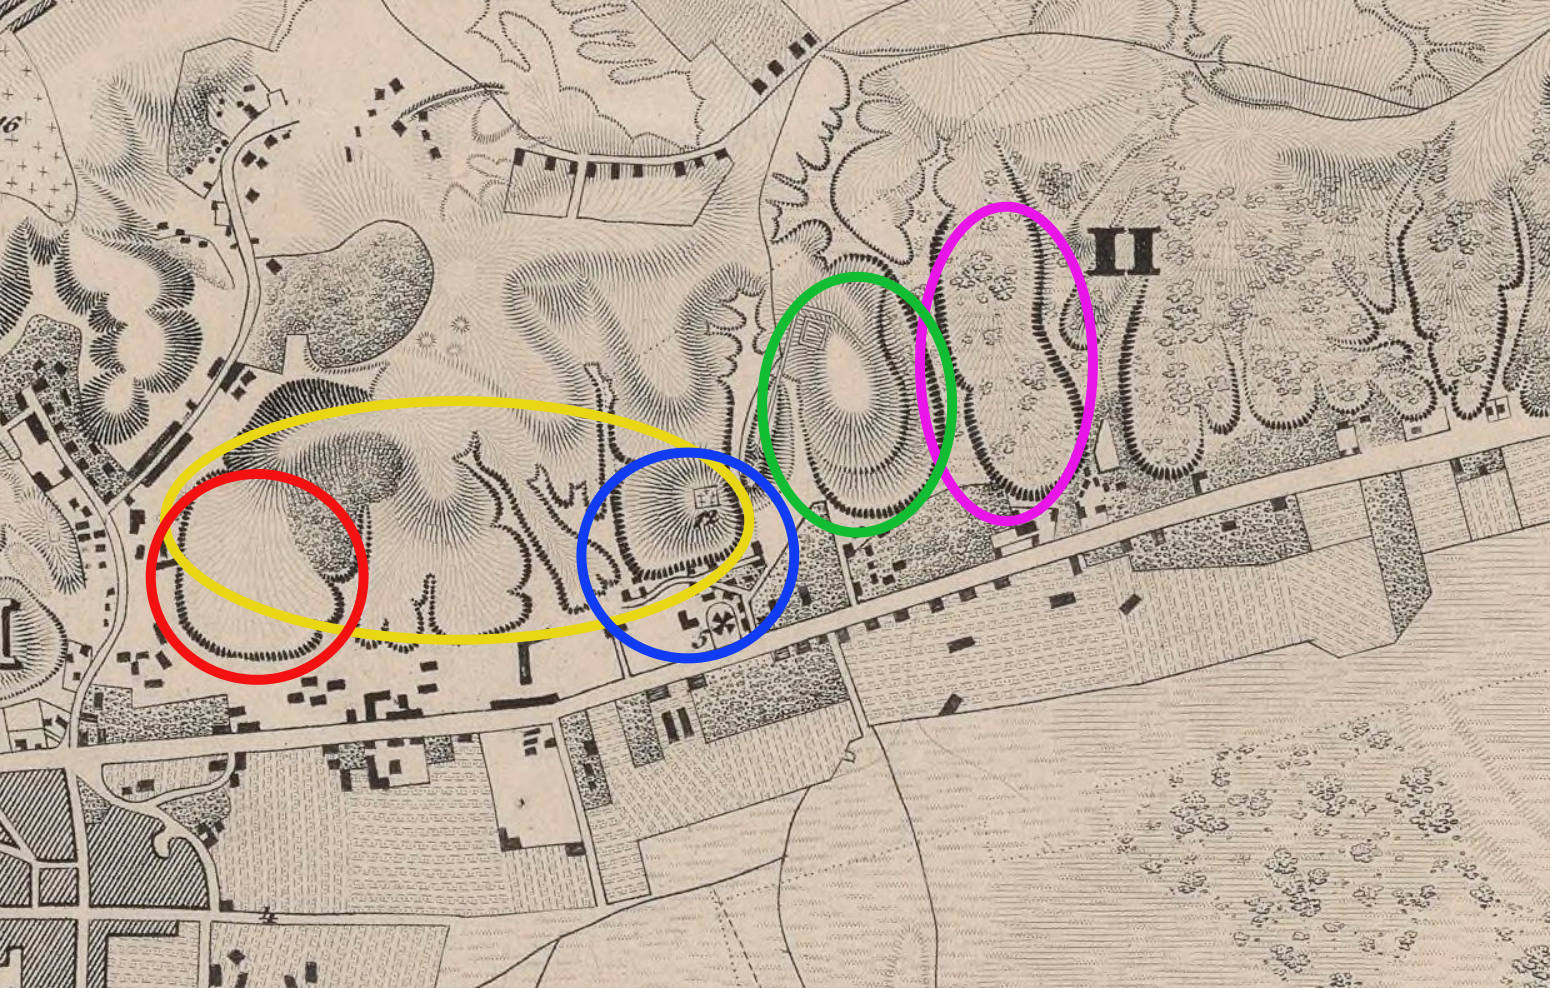
\includegraphics[width=\linewidth]{chast-kirvys/kirstoy/1845-vmap.jpg}
\end{center}

Горизонтальная большая улица – это Кирилловская. Желтый овал – Лысая гора, «новая» Юрковица. Красный – сожранный кирпичным заводом ее юго-восточ\-ный отрог, это там сейчас военная часть и завод. Да и правее (северо-западнее) от тела холма остались рожки да ножки. Синий – это, внизу старая Иорданская церковь (теперь место нотной фабрики), а наверху отрог Лысой горы с Иорданским кладбищем. Зеленый – отрог «Кожевника». Малиновый – уничтоженный отрог с Кирилловской стоянкой.

В конце августа 1893 года Хвойка осматривал усадьбу Зиваля (имела адрес Кирилловская улица, 59) и обратил внимание на знаменитый впоследствии отрог горы. В северном склоне, заросшем деревьями и кустами, Хвойка заметил несколько мест, где добывали глину, и решил поглядеть там из каких слоев грунта состоит холм. 

В самом нижнем слое, «серо-зеленоватых мелкозернистых песков», Хвойка увидел правильный желто-белый круг. С этого всё и началось. При небольшом раскопе вглубь круг оказался бивнем мамонта. Хвойка не спешил рыть дальше, а тем паче хвататься за бивень и пытаться его вытащить. Он смекнул, что рядом могут быть еще другие древние кости, и что без тщательных раскопок не обойтись.

Хвойка договорился о них с Зивалем, и на следующий день приступил к раскопкам. Бивень крепился к остаткам огромного мамонтового черепа. Хвойка снова проявил осторожность и обратился за советом к Владимиру Антоновичу. Тот приехал на место, сообща решили продолжать. 

День спустя Хвойка, уже при помощи рабочих, начал более масштабные раскопки. Ничего. Еще через день удалось найти второй бивень и нижнюю, недостающую часть черепа. Пока Хвойка очищал кости от земли, рабочий обнаружил кремневое орудие. Археолог отложил работу с черепом и в месте, указанном рабочим, наткнулся еще на два сходных орудия труда.

Сопоставив наличие костей мамонта в одном культурном слое с орудиями труда, Хвойка решил, что это доказывает «совместное существование человека и мамонта», а орудия отнес к эпохе палеолита. Осознавая важность открытия, снова послал весть профессору Антоновичу. Он прибыл спустя три дня вместе с профессором Петром Армашевским. За это время Хвойка откопал еще пять кремневых предметов.

Армашевский – геолог, сторонник высшего женского образования, защиты животных, любитель природы, монархист. Это он разработал сеть артезианских колодцев Киева, а также систему штолен на Владимирской горке, для отвода грунтовых вод и предотвращения оползней. В первых числах мая 1919 года был расстрелян как контрреволюционер. Контрреволюционер в последние годы жизни сидел в кабинете и работал над курсом кристаллографии.

\begin{center}
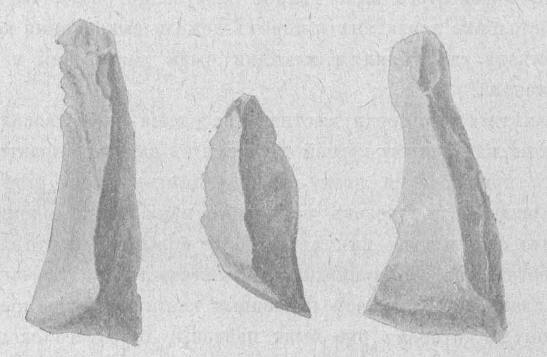
\includegraphics[width=0.70\linewidth]{chast-kirvys/kirstoy/1893-hvoyka-kremen-01.jpg}

\textit{Первые три кремневые орудия, найденные на Кирилловской стоянке.}
\end{center}

Армашевский стал часто посещать продолжившиеся раскопки Хвойки. Но случилась беда. 

На место повалили киевляне, падкие на зрелища. Нашли кости мамонта! Каменные ножи и стрелы! В ближайшие выходные явилась толпа зевак. Сторож выдворил их прочь из усадьбы, запер ворота на замок, но люди впали в неистовство и прорвались внутрь. Хвойка оставлял кости на столбиках земли, чтобы не нарушать порядок... Всё это было сметено, растащено, украдено. Подоспевший к окончанию разграбления Хвойка столкнулся со старухой, собиравшей древние кости в узелок. Все мол знают, что кость мамонта – целебная. Для того, дескать, Хвойка и проводит раскопки.

Хвойка решил более не рисковать, а зарисовывать и фотографировать находки на месте обнаружения и затем их прятать. Но фотосъемку получилось провести лишь пару раз, чтобы запечатлеть «некоторые части и общий вид раскопок».

Из года в год Хвойка продолжал работы. В то же время усадьбы Зиваля и Багреева (тогдашний адрес – Кирилловская, 61) купил Иона Зайцев, для постройки большого кирпичного завода – надо думать, на основе уже существующего предприятия Багреева. 

Для доступа к синей глине под отрогом Кирилловской стоянки Зайцеву понадобилось срыть почти весь отрог. За делом наблюдал, делая раскопки, Хвойка. Это позволило досконально изучить холм, но уничтожило древнейший памятник первобытной жизни. На месте отрога возникло так называемое «глинище» – карьер по добыче глины, а комплекс переработки расположился наверху холма.

Еще ниже глинища, к востоку, Зайцев выстроил еврейскую больницу – позже при ней, под видом столовой – молельный дом, что открылось на суде по делу Бейлиса, ибо на молельный дом разрешения властей не было. Больница эта и стала потом, в 1949 году, Подольским роддомом.

В 1893 году Хвойка сделал следующую зарисовку слоев еще относительно целого тогда мыса:

\begin{center}
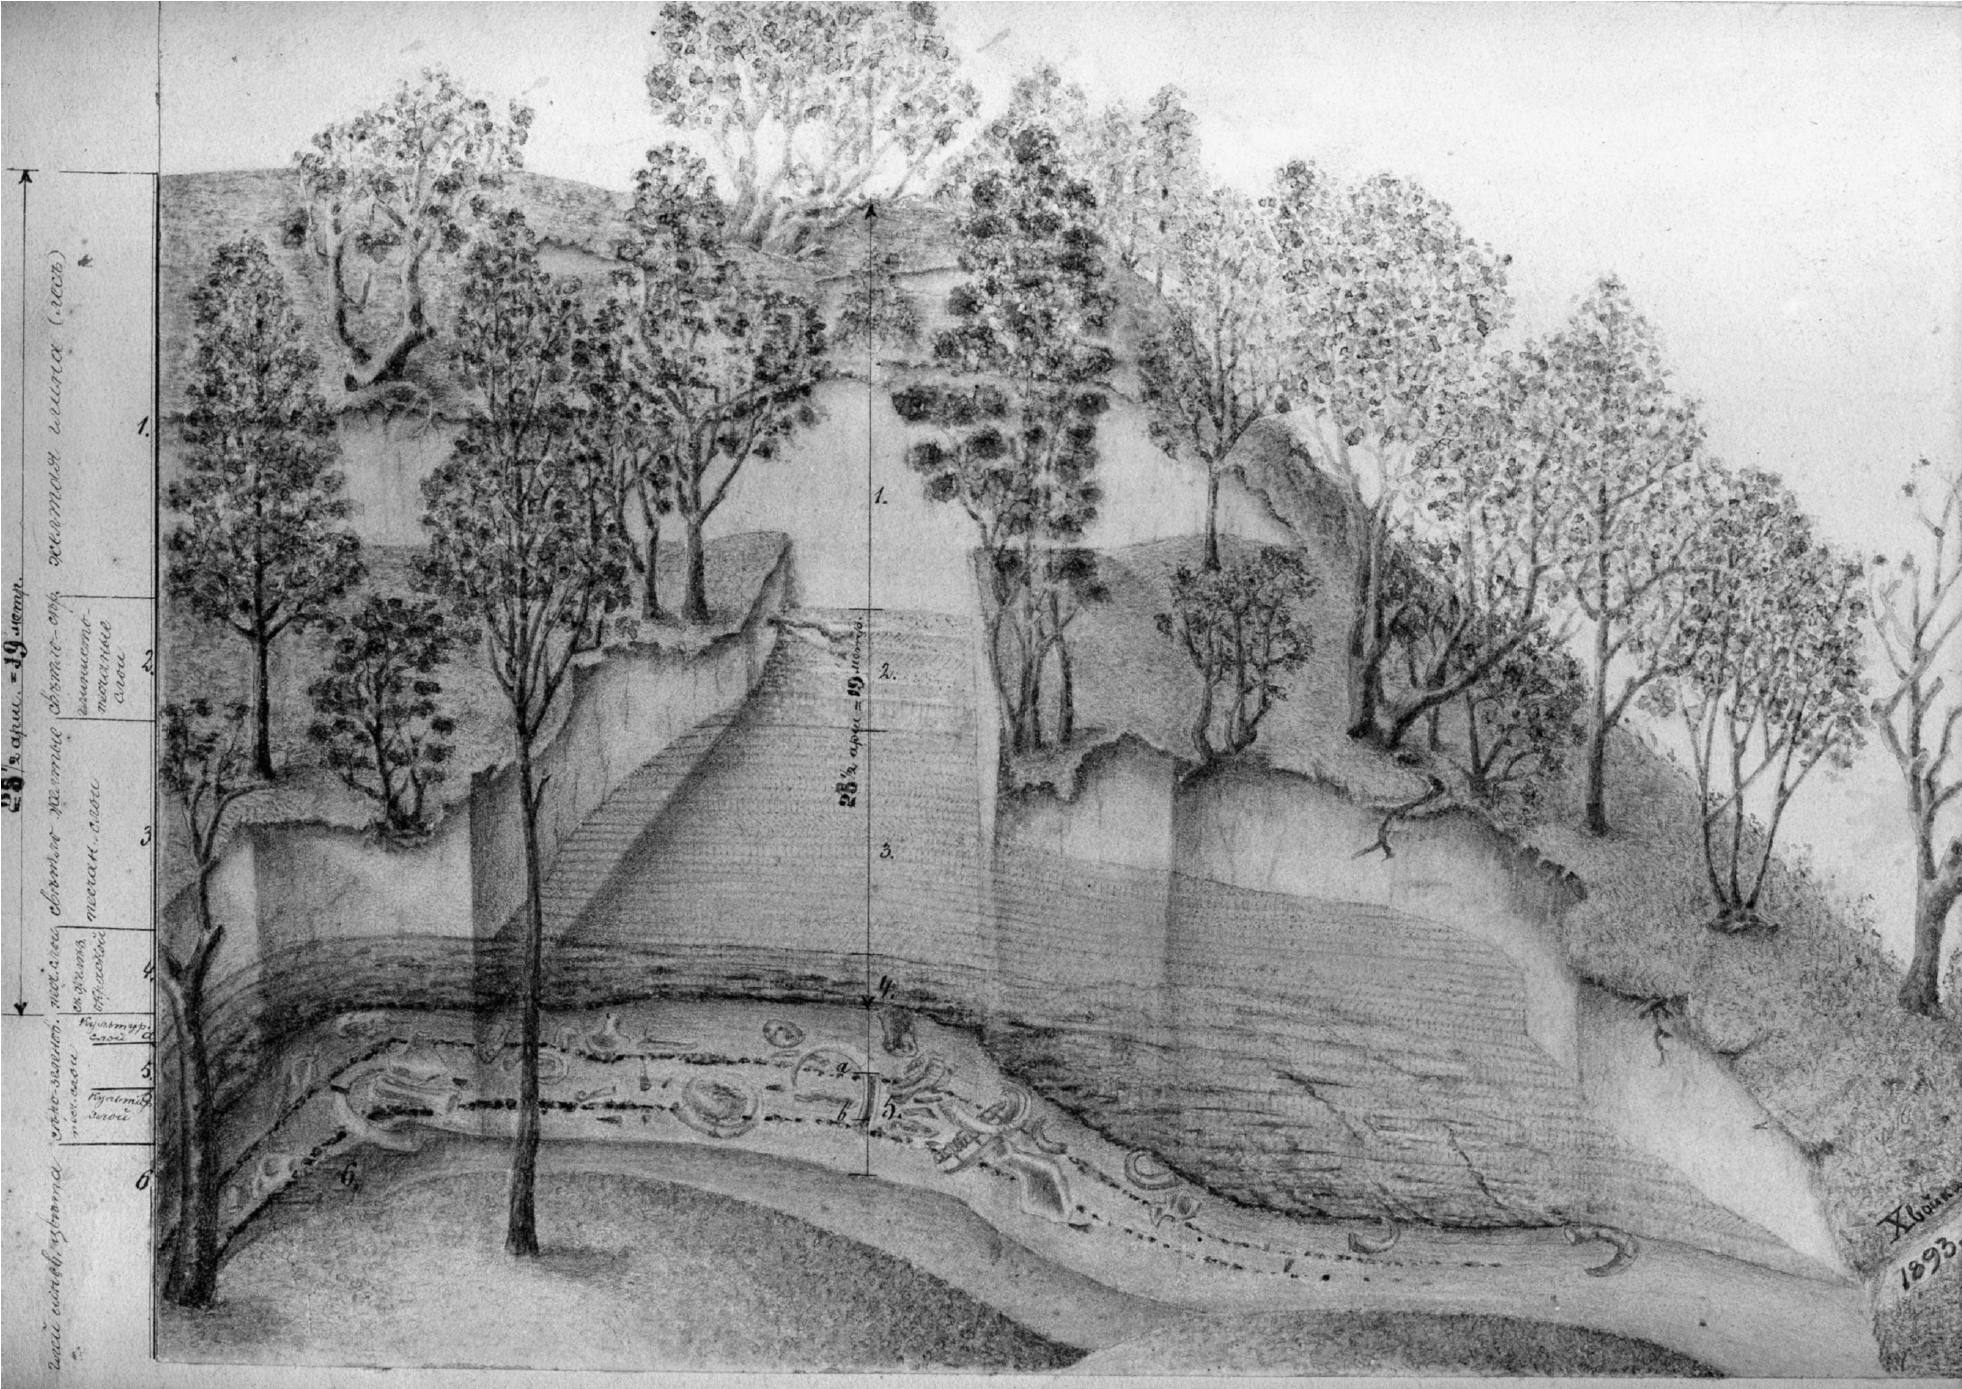
\includegraphics[width=\linewidth]{chast-kirvys/kirstoy/1893-hvoyka-03-2.jpg}
\end{center}

1 – лёсс; 2 – светло-серые глинисто-песчаные слои; 3 – светло-желтые песчаные слои; 4 – песчаные слои с желтой окраской; 5 – серо-зеленые песчаные слои с культурным слоем; 6 – глей синеватого цвета.

Следующий «послойный» рисунок Хвойка сделал в 1894 или 1895 годах:
\vspace*{\fill}
\begin{center}
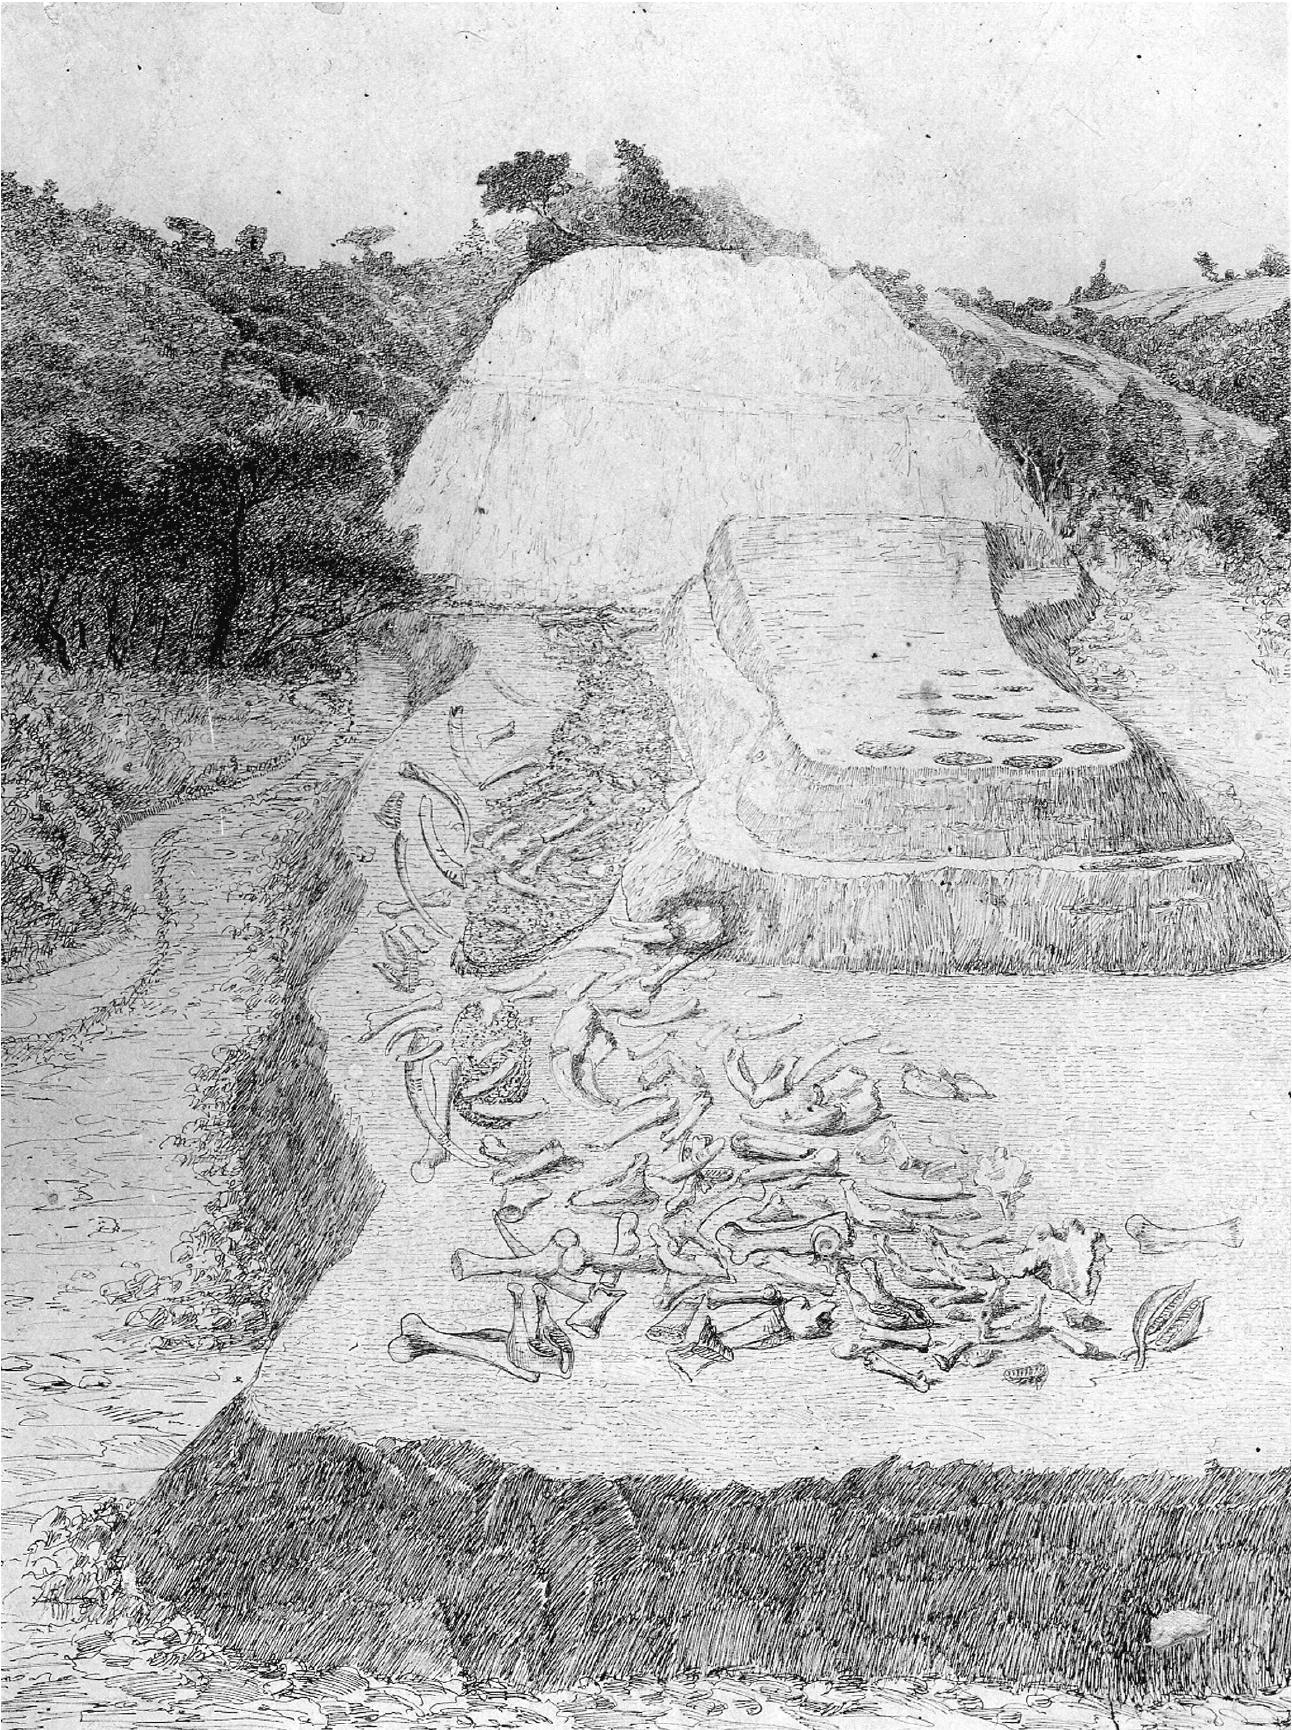
\includegraphics[width=\linewidth]{chast-kirvys/kirstoy/1894-hvoyka-01-01.jpg}
\end{center}
\vspace*{\fill}
\newpage

Под завершение раскопок, когда холм был уничтожен, была сделана окончательная геологическая роспись слоев:

\begin{center}
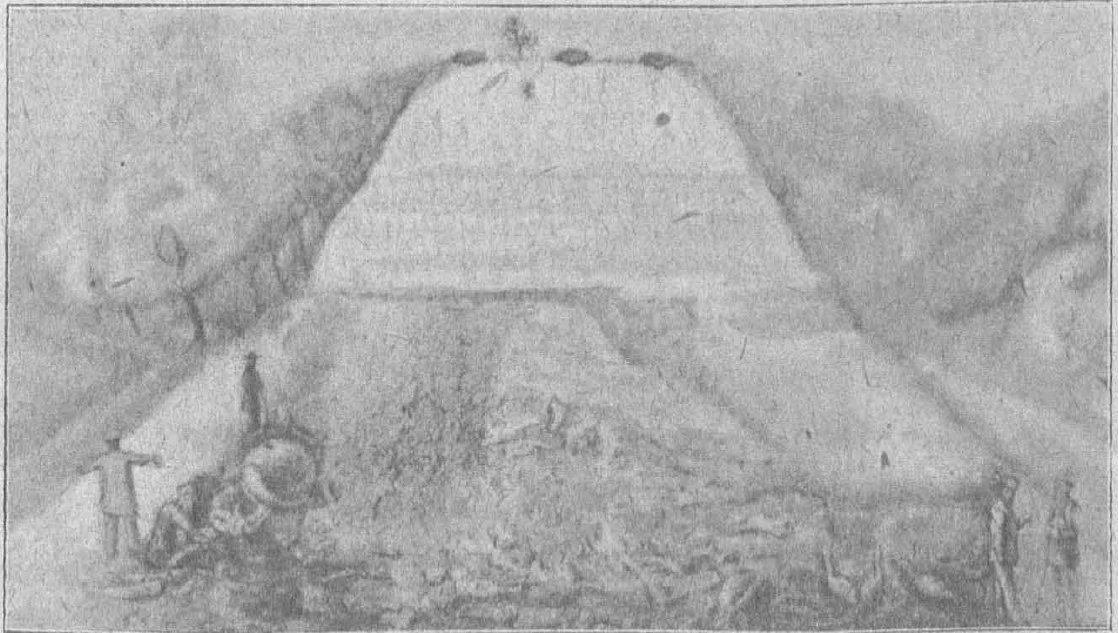
\includegraphics[width=\linewidth]{chast-kirvys/kirstoy/1899-hvoyka-01.jpg}
\end{center}

Данные таковы, сверху вниз:

лёсс – 10 м.

суглинок – 1,5 м.

слоистые пески – 6 м.

железистый песчаник, слой валунов, и железистых сростков – 1,5 м.

серо-зеленоватые пески – 1 м.

Вот теперь можно порассуждать о слоях культурных! Хотя в литературе обычно говорят только о двух слоях, «нижнем и верхнем», не всё так просто.

Наиболее глубоко, в синей глине, но в 120 метрах от первой находки, на глубине 21 метра Хвойка нашел несколько костей и нижних челюстей мамонта, череп носорога с зубами в верхней челюсти, молодого мамонта бивень длиной 1 метр 70 сантиметров – с желобком 4 см. ширины и 3 см. глубины по всему протяжению, с зарубками по краям, лежащие рядом части стволов кедра со следами огня, и кусок бивня с вырезанными изображениями, в коих Хвойка усмотрел «какое-то щитоносное животное в виде черепахи, птичью голову и нечто в виде ладьи».

\newpage

Вот фотографии этого бивня и рисунок с развернутым на плоскости узором:

\begin{center}
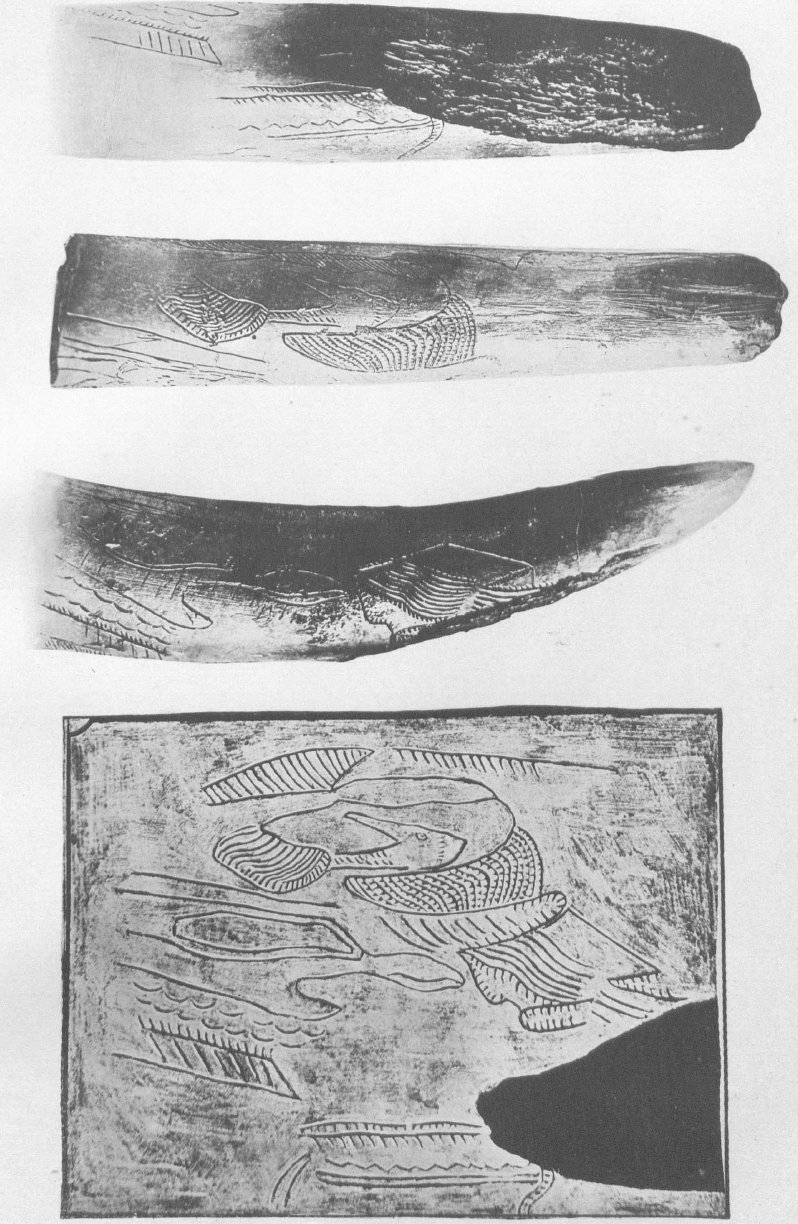
\includegraphics[width=\linewidth]{chast-kirvys/kirstoy/1893-hvoyka-biven-01.jpg}
\end{center}

\newpage

Мне сложно судить, что изображено, с какой целью использовался такой украшенный бивень, и сколько времени и труда ушло на работу. Чем её выполнили – кремневым орудием? Есть много трактовок сюжета гравюры – от бытовых до мистических и календарных. Я не буду их касаться. Очевидно, что узор нанесен со смыслом.

А ведь это сделано во время, когда под рукой были, вероятно, только огонь, кремень и кости. Хорошо, допустим, выцарапали кремневым ножом. Неандертальцы, например, делали столь острые ножи, что ими до сих пор можно бриться. Но кроме технологии, само содержание рисунка-узора приводит к ряду выводов.

Художник знал счёт и имел представление об углах. Использовал линии прямые, пилообразные. Кривые. Некоторые объекты изображены им с четкими ровными контурами – например, левый нижний объект на развернутом рисунке, напоминающий конвейер, над которым 2 ряда по 7 дуг в каждом.

Объекты такой формы не должны были встречаться среди той дикости, в которой, как считается, пребывали первобытные люди, «охотники на мамонтов». Не должны были существовать! Тогда что же изобразил мастер? Может, мы чего-то не знаем о том, древнем мире? Или рисунок несет прикладное значение – например, это карта, календарь, счеты, либо даже письмена?

Над синей глиной, в толще горы, в серо-зеленоватых песках, Хвойка нашел еще три культурных слоя, отнесенных им к палеолиту. В первом, нижнем, в усадьбе Зиваля, лежали кости, бивни мамонта и прочих животных. Кремниевые орудия были не между костями, а отдельно. Бивни с зарубками на концах, некоторые обожжены.

Чем дальше Хвойка углублялся в гору, тем меньше попадалось ему костей, однако стали появляться угли да куски окаменевшего дерева. Наконец докопался до сплошного слоя «кострища», местами метровой толщины. Зола, уголь, разбитые кости мамонта и других зверей, «как бы нарочно сложенные». Все они были обуглены и редко удавалось достать их целыми – рассыпались в руках. Неподалеку, но 70 сантиметрами ниже, Хвойка наткнулся на второй такой пожарищный слой. Есть свидетельство Хвойки о том, что именно во втором слое ему попалось много кремневых орудий – с другой стороны, Хвойка же пишет, что кремневые орудия никогда не находились непосредственно среди костей и угля, но лежали «ниже верхней полосы и крупных костей, а иногда на самой поверхности синей глины». Могу заключить разве что кремневые предметы были между синей глиной и углем.

\begin{center}
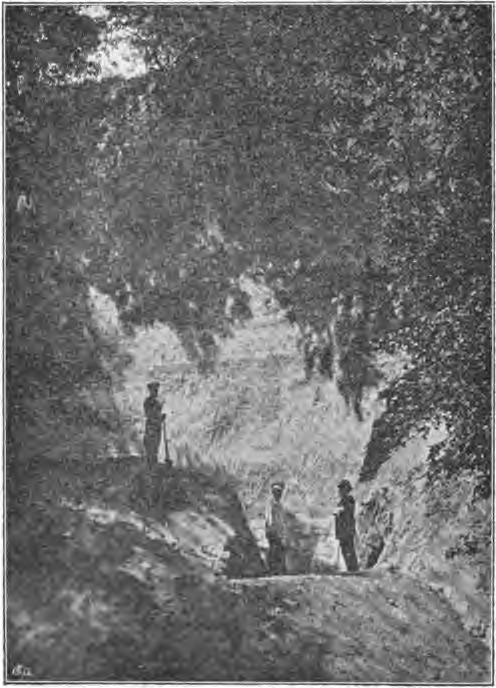
\includegraphics[width=0.60\linewidth]{chast-kirvys/kirstoy/hv-rask.png}

\textit{Плохой скан снимка с раскопок Хвойки.}
\end{center}

В глубинных слоях, Хвойка выкопал более 50 нижних челюстей мамонта и приблизительно 100 бивней, не считая обожженных из кострища. Некоторые бивни выглядели подобно дубинкам – толстая часть скруглена, тонкая сточена в форме рукоятки. Кремневых орудий же отыскали примерно 200.

Продолжив раскопки уже в части отрога, принадлежащей Багрееву (Кирилловская, 61), Хвойка обнаружил на глубине 13-14 метров от поверхности земли, «под пластами бурых слоистых суглинков», две, лежащие в метре одна от другой, полосы нового культурного слоя. Их содержимое археолог описал как круглые и овальные площадки в виде гнезд диаметром около 2 метра каждое. Площади были на разной высоте – метр туда, метр сюда.

Гнездо – значит, стащили сюда предметы, как птица всячину в гнездо приносит и раскладывает. Условность. Наши ученые в 20 веке взамен этого придумали другое, неуклюжее – «очажное топталище». Наверное имели в виду, что тут, на пятачке 2 метра в диаметре, из года в год топтались первобытные люди. Соорудили очаг и топчутся в нем.

Всего Хвойка насчитал около 20 «гнезд» на площади 30х20 метров. В них лежали измельченные кости мелких животных, редко – мамонта (и то на нижней площадке), а также челюсть и часть черепа пещерного льва (по Хвойке, а профессор Армашевский назвал это животное ископаемой кошкой размером со льва), челюсть пещерной гиены, зубы пещерного медведя.

Кремневые орудия числом свыше 3000, более совершенные, чем на «мамонтовом» слое, нуклеусы (остатки, основы камней, от которых откололи куски для изготовления орудий), кучи необработанных кремней. Последнее вызывает недоумение, ведь извлеченный на воздух, обсохший кремень быстро теряет свои качества «обрабатываемости» и становится бесполезным для откола от него длинных кусков. Иными словами, заготавливать кучи кремня впрок – напрасный труд.

Эти культурные слои относились к палеолиту, однако наверху холма, на площади 4000 квадратных метров, на глубине от 40 сантиметров, Хвойка отыскал и неолитической культурный слой! Именно находки в этом слое отмечены Хвойкой на плане горы с ракурсом «вид сверху», два варианта которого я привел несколькими страницами раньше. 48 ям-раскопов дали представление о неолитическом слое.

От чернозема он уходил глубже, в лёсс. Вначале, ближе к поверхности, Хвойке попадались черепки керамики, обломки костей, речные ракушки Anio pictorum и Anodonta cygnaea, уголь, зола. Потом в лёссе были отрыты остатки пещер, не менее шести. В одной – ниша с обожженными докрасна стенами. Нечто вроде печи Хвойка нашел в другом месте, причем для строительства были использованы глина, камень, щебень, прутья, колья.

Чем дальше от середины горы, тем глубже были пещерки, и тем примитивней набор предметов в них – это касается набора костей, орнаментов на керамике и так далее. А чем ближе к середине, тем меньше ракушек, выше качество и сложность керамики. Получается, что вырытые ближе к склонам пещеры постепенно оставлялись в пользу более новых, тяготеющих к центру. Почему?

Кроме пещер, в ходе раскопок Хвойка встретил площадки из обожженной глины. Конечно же, подземелья и площадки не были пустыми. Сначала о костях. Хвойка нашел три человеческих скелета, один ростом 1,85 метра. Однако Хвойка считал, что они попали туда позже, не являлись современниками пещер. Также лежали кости рыб, птиц, кости и зубы млекопитающих, из коих археолог упомянул бобра, оленя, волка, дикую козу. Панцири пресноводной черепахи валялись на полу. Были и ракушки – они измельчались в муку, добавляемую в глину для лепки посуды.

Предметы. Кремневые, роговые и костяные орудия – ножи, топорики (в том числе из рога лося и оленя), скребки, долота – причем с орнаментами, и тому подобное. Два глиняных прясла с орнаментом, костяное шило. Шлифованные куски песчаника. Глиняные бусины. Обломок фигурки из темно-красной глины.

Глиняная обожженная посуда. Миски, причем выкрашенные. Горшки с ушками. Покрытые узором горшки разных видов – с толстыми стенками и тонкими. Хвойка пишет:

\begin{quotation}
Один из таких сосудов по форме напоминавший амфору, был сделан из красной глины и поверхность его была так хорошо сглажена, что блестела как лакированная. 
\end{quotation}

\newpage
\vspace*{\fill}
\begin{center}
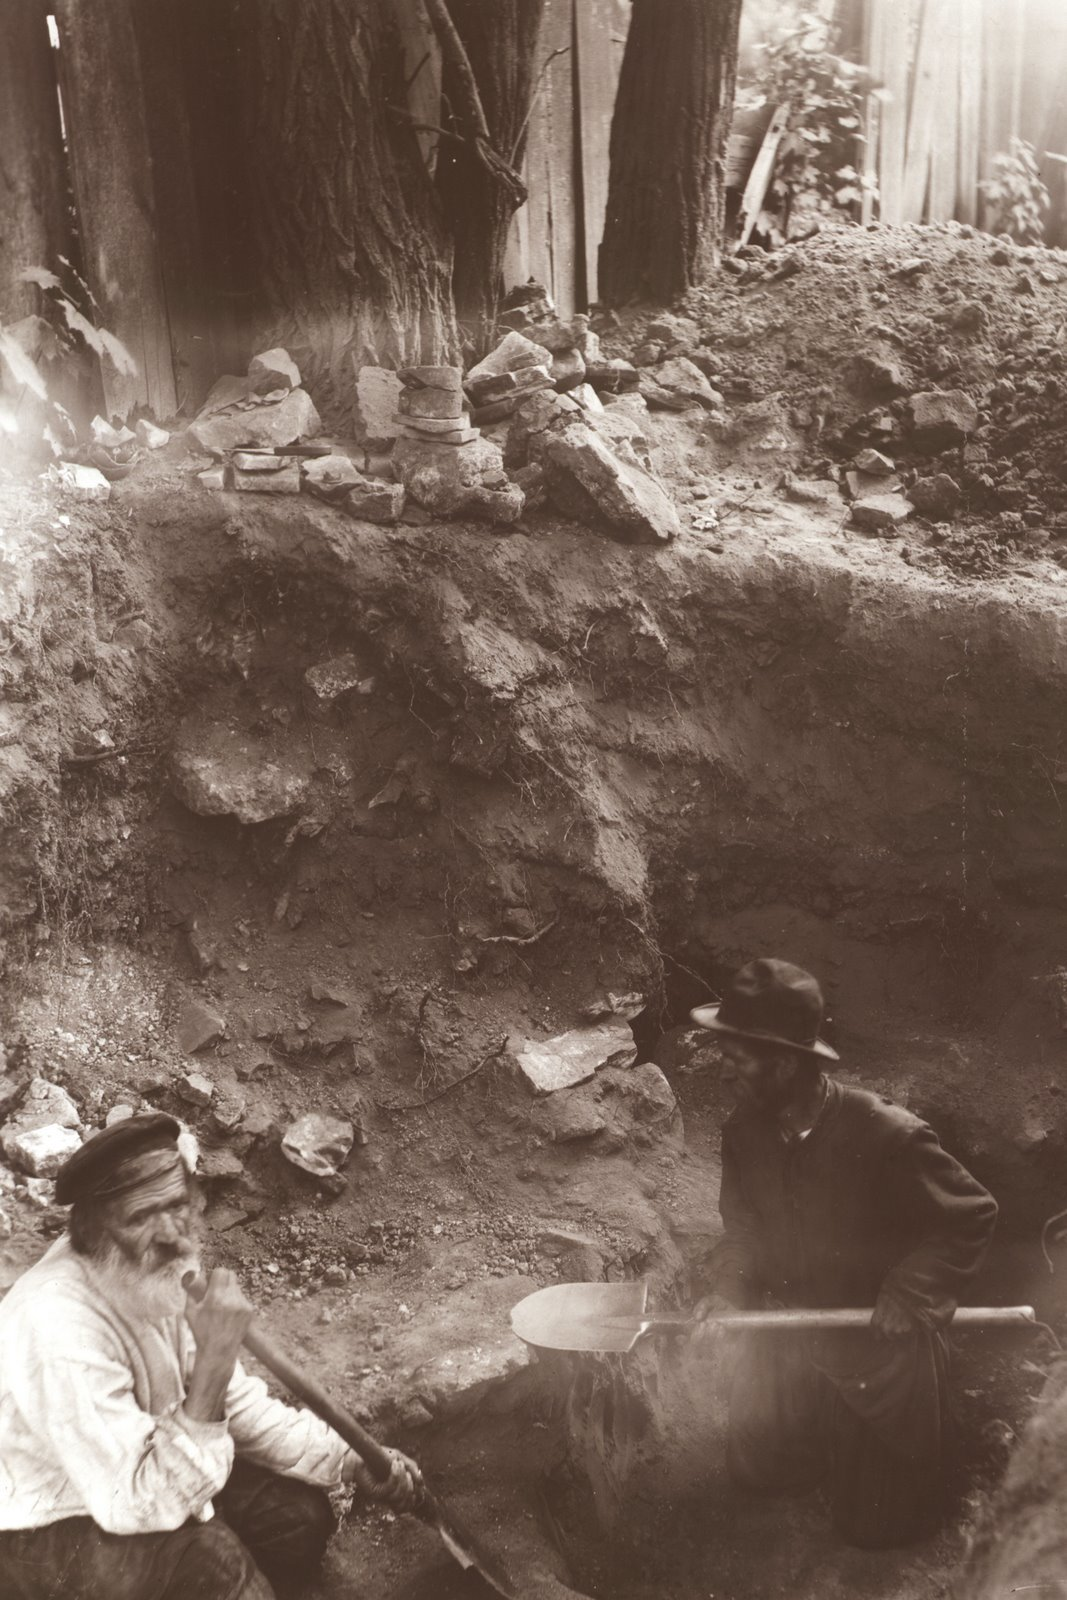
\includegraphics[width=\linewidth]{chast-kirvys/kirstoy/hvoyka-03.jpg}

\textit{Отличный скан снимка с раскопок Хвойки.}
\end{center}
\vspace*{\fill}
\newpage

Некоторые сосуды были докрасна обожжены. Узоры напоминают елочку и другое рифление современных велосипедных и автомобильных покрышек.

Пища. Ракушки, кости животных дают основания полагать, что обитатели верха горы поначалу ели моллюсков, а затем освоили рыболовство и охоту. Хвойка обратил внимание на окаменевшие лепешки с косточками, как бы поджаренные.   

Необычное. Нашли глиняную формочку для отливки, как предположил Хвойка, медных или бронзовых топориков. Прототип из рога лежал тут же. Формочка состояла из двух половинок, и роговой топорик вписался в них. Однако металлических изделий в месте раскопок нигде не обнаружили. Но ведь под боком – какой-никакой, а слой железистого песка вперемежку с кусками железной руды. Однако литье именно железа возможно при температуре от 1530 градусов, и считается, что лить железо научились только с изобретением в 19 веке доменных печей. Но что, если гораздо раньше?

О трактовке находок в горе. Хвойка, Антонович и Армашевский полагали Кирилловскую стоянку древнейшей в Российской империи, давали нижнему её культурному слою по меньшей мере 20000 лет.

Слой, где были обильны бивни и кости мамонта, считался Хвойкой отделенным от «гнездового» слоя большим промежутком времени – и относительно небольшим промежутком пространства. Во втором слое мамонт уже вымер или стал редкостью. Хвойка утверждал, что люди, к которым относился нижний слой, охотились на неповоротливого мамонта, который был одним из немногих доступных им видов дичи.

Как же случилось, что над всеми этими бивнями, костями и орудиями возникла целая гора? По Хвойке, стоянка располагалась в местности еще без гор, полной озер котловине у большой реки, вероятно первобытного Днепра. Тут росли высокие кедры и ели, бродили мамонты. Но с севера подступал ледник, из-под которого вода несла грунт, постепенно заполняя наносами долину Днепра, пока она не переполнилась. Тогда вода выступила над уровнем долины, затапливая окрестности. Ледник надвинулся, затем начал таять, отступать к северу. Снова наносы. Река пробила себе новое русло уже в них, уровень дна снизился.

Слои песка между культурными слоями, как полагал Хвойка, означают несколько затоплений местности, во время которых грунтовые наносы покрывали предшествующий культурный слой. Таким образом, «гнездовой» слой относится ко времени, когда растительный и животный мир здесь сменился, прошла эпоха мамонтов и вооруженных палицами первобытных людей, люди стали более изобретательны и смертоносны. Наконец, толстый слой лёсса от песков и выше, до хилой шапки чернозема, означает длительное затопление и последующие намывы.

Еще в 19 веке Хвойке возражали, говоря, что в разрезе холма нет морены – валунной глины, которая должна присутствовать, если местность была покрыта ледником, и поэтому Кирилловской стоянке надо определить возраст не более 12 тысяч лет, когда, как считается, завершился последний ледниковый период. Что до образования лёсса, то существует другая гипотеза, что не от намыва получился лёсс, а ветром надуло.

Я не геолог, поэтому не буду пускаться в рассуждения. Меня убеждает мысль, что раз отрог со стоянкой укрыт, будто сугробом, равномерным слоем лёсса, это значит, что гора выросла, выростала над всеми подлежащими культурными слоями. Самый нижний из коих по странному совпадению находится примерно на современном уровне воды в Днепре. Лёсс мог возникнуть и как последствие Всемирного потопа.

Итак – гор\'ы, по представлениям Хвойки, во время мамонтов не было! Отдельные ученые 20 века, например Пидопличко в своей работе 1969 года «Позднепалеолитические жилища на Украине», да и другие того же времени утверждали, что стоянка лежала у склона высоченного правого берега, и 22 метра лёсса над стоянкой ветром надуло, со склона.

Куда же делась потом эта огромная, выше нынешней, гора правого берега? Её всю сдуло точно до уровня выступающих отрогов? Всю эту массу грунта? А лабиринт узких и высоких отрогов, тоже покрытых лёссом, к северу от Совской балки – с какого массивного правого берега их надуло? Они там существуют будто сами по себе.

А вообще были тогда, в древности Киева горы, большие возвышенности? Это вопрос важный. Нам же рисуют на картинках в популярных книжках по археологии, как первобытные люди охотились на мамонта. Загоняли несчастное животное на край обрыва, оно падало и гибло. Но если гор не существовало, какой обрыв? Про горы в Киеве есть разные мнения. Противоположные. По одному, говоря басенным слогом, и горы были выше, и реки глубже. По другому – до приближения ледника высота гор была метров на 30 меньше.

Хорошо бы на машине времени отправиться и поглядеть, что к чему. А без этого можно выдвигать сотни предположений, на ходу придумывая вспоможения для обоснований. Нужна гора под самое небо – пожалуйста. Теперь будет, с чего сдувать и образовывать лёсс. А может и была гора, черт его знает.

Хвойке задавали вопрос – как же охотились на мамонта, если найденные на стоянке кремневые орудия явно мелковаты, чтобы справиться с мохнатым великаном? Этими орудиями и яму для поимки мамонта не выкопаешь. Хвойка ничего толком не ответил, кроме утверждения, что древний человек питался мамонтом, без мамонта не мог существовать, а другие более подвижные животные были недоступны оружию.

Дык как же, если кремневые скребки или даже дубины из бивней против мамонта – жалкое средство борьбы? Да и, думаю, мамонт был чертовски проворен. Напротив, для охотника он должен быть наиболее сложным видом добычи.

Всё, что нашел Хвойка в нижнем слое – мамонтовые кости, бивни и мелкие кремневые орудия. Никаких человеческих костей. А ведь хозяева кремневых орудий просто могли приходить на эдакое мамонтовое кладбище, как существуют загадочные кладбища слонов. Искали кости, годные в качестве дубинок, прочего оружия.

Никаких явных следов жилья.

Как!? А знаменитые жилища первобытного человека, сложенные из бивней, костей и черепов, да обтянутые шкурами? На картинах, рисунках, в фильмах, мультфильмах нам их показывают уже много лет. Они же стоят в некоторых музеях.

Ну так в основание ученые впихнули металлические каркасы, потому и стоят. Не будет каркаса – стоять не будут. 

Археологи, в частности сторонник идеи «костных жилищ», Иван Пидопличко, оценивал вес сооружения из костей и шкур в три тонны, и развивал мысль дальше – для каркаса использовались деревянные жерди, но основной вес держал на себе цоколь из черепов и трубчатых костей. Правда, жердей никто не нашел, а цоколи из черепов – в самом деле, в некоторых местностях ученые раскопали кости и черепа, разложенные в определенном порядке, например по кругу. Что с того? Такой порядок мог быть обусловлен ритуальным назначением. При чем тут жилье?

Хибара из мамонтовых костей гораздо менее пригодна для обитания, чем нора хоббита. Вообразите себе сложность самого сооружения! И его прочность. Если обвалится, то жителей здорово прихлопнет костомахами. И сами кости – если только под рукой не было огромных запасов старых, полностью очищенных от мяса костей – надо было чем-то выскоблить, ведь не строить же из падали.

В чем же удобнее было жить? В пещерах или норах. В дуплах. Вспомним отшельников! Уходили от мира, копали себе пещерку и жили. Нора – самое понятное дело, все звери себе роют. А пещеры бывают и естественные, если повезет. Конечно, коли грунт не позволяет рыть хотя бы землянку, то надо строить на поверхности. Но и тогда для этого более пригодна древесина, нежели кость. А если древесины нет? Но тогда и хижина из костей стоять не будет, рухнет с первого пинка.

Эдак до середины 20 века в ученой среде не говорили о мамонтовых хижинах. Потом украинские ученые в кучах костей усмотрели остатки хижин, и пошло-поехало. С тех пор их «нашли» на Украине, в Молдавии, Польше и Чехии. Американские ученые решили – что мы, хуже? Вдруг оказалось – древние индейцы охотились на мамонта и строили костяные халабуды. В американских музеях стоят реконструкции «мамонтовых хат», в них любят фотографироваться дети. К хатам приставлены манекены первобытных индейцев.

Но вернемся к Кирилловской стоянке. Нынче некоторые археологи считают, что нижний «мамонтовый» слой и более верхний «гнездовой» – это один и тот же слой. Но из самого состава найденных в этих слоях предметов вывод напрашивается противоположный.

Далее, явных следов жилья и во втором слое нет. Зола... Ну люди и сейчас выезжают в лес, жгут костры – это не значит, что они живут на месте пикника. А вот найденное Хвойкой кострище вызывает вопросы. Огромный пожар? И что сгорело?

А почему надо предполагать, что владельцы всех этих кремневых орудий – именно люди, представители рода «человек разумный», его родичей или предков? Мы ведь не знаем, кто именно притащил сюда эти предметы. Мы не знаем, по какой причине погибли мамонты, чьи кости тут лежат. Убиты или умерли сами? Ответа нет.

Хорошо, но кто, кроме людей, мог проявить себя? Для меня нет внутреннего барьера допустить существование иных биологических видов, способных производить орудия. А много ли будет найдено останков, если такой вид относится к паукам или каким-нибудь сухопутным моллюскам со щупальцами? Они же полностью разложатся.

В одном культурном слое есть кремневые орудия и костные дубины, есть кости мамонтов. Я не могу логически вывести из этого, что орудия и дубины принадлежали людям. Нет оснований. Возьмем те же две гипотезы возникновения лёсса. Ветром или намывом? Обе гипотезы можно вроде бы и доказать, и опровергнуть. Или – ни точно доказать, ни точно опровергнуть. Так что же, обе верны? Одна ложна? Обе ложны? 

Кости мамонта и кремневые орудия? Мамонт не дурак и у него есть хобот. Известно, что слоны умеют использовать инструменты. Например, берут хоботом палки и чешут себе спину. Или – отламывают ветку с листьями и отгоняют насекомых. Слоны рисуют картины – под руководством человека, но рисуют. Что мы знаем об умственном уровне развития мамонтов? Ничего. Связка мамонтов и орудий труда более обоснована, чем связка с третьей составляющей – людьми, чьих непосредственных следов ни в одном из глубинных слоев не найдено. Я не говорю, что так было. Я говорю про основания для суждений.

Кости мамонтов в нижнем слое. Положим, там кости до сотни особей. За какой срок они умерли? Существующие средства датировки не позволяют это вычислить. Ответ на вопрос дал бы зацепку для распутывания загадки. Хотя, для ученых и журналистов загадки нет, есть «стоянка», населенная первобытными охотниками на мамонтов. Костяные хижины и всё такое. Все всё знают и ничего больше не нужно.

Кстати, кости мамонтов находили в разных частях Киева. Только в 19 веке их, вымытыми дождями, обнаруживали в Кирилловском овраге (западный отрог того, что ныне слывет как весь Репяхов яр), в овраге у Байковой горы, а на Вознесенском спуске сыскался целый череп и также несколько костей.

Собирая сведения о Кирилловской стоянке, я наткнулся в одном из весенне-летних томов «Киевской старины» за 1899 год на заметку с важнейшими подробностями, умолчанными в других известных мне источниках:
 
\begin{quotation}
Исследования стоянки палеолитической эпохи, обнаруженной в усадьбе Зайцева, по Кирилловской улице в городе Киеве, продолжались в течение всей истекшей зимы и начала весны. За последнее время обнаружена масса костей, главным образом мамонта, следы кострищ и отбивные кремневые орудия.

При съеме верхней части горы, у подошвы которой лежит палеолитическая стоянка, открыта пещера, вырытая в лёсе, имевшая 75 стм. в вышину. На стене этой пещеры обнаружены какие-то знаки, имеющие вид письмен.

Пока трудно еще решить к какому времени относятся эти знаки; пещеры в лёсе, каковыми изобилует нагорный берег днепровской долины, служили жилищем первобытному человеку неолитической эпохи каменного века, – немножко смело относить к этой эпохе и новооткрытые «письмена»; нужно иметь в виду, что пещерами этими, особенно в раионе г. Киева, зачастую пользовались и в позднейшее время, так например их приспособляли для целей пустынножительства, предварительно конечно расширив, давали оне приют и разному бездомному люду и в самое последнее время: несколько лет тому назад, при осмотре такого рода пещер, лежащих пососедству с вышеописанной, в одной из них мы набрели на остатки, имеющие мало общего с археологией; тут валялись бутылка от водки, объедки, какие-то тряпки и т.п. – повидимому следы недавнего пиршества после дележки.
\end{quotation}

Что это? Обнаружена пещера, возможно с древнейшими письменами! При срытии склона – надо думать, подземелье затем похерили устроением завода Ионы Мордковича Зайцева, уничтожившего тут навечно все исторические памятники.

Древнейшие письмена! Им уделена короткая заметка, без иллюстрации, без подробного описания пещеры. Где именно она располагалась, какие размеры и строение имела? В лёсе... Какие-то знаки... Сочинитель лучше про бутылку водки напишет, чем уделит лишнюю строчку главной находке. Хоть бы перерисовали письмена, абзацем тиснуть – нетрудно!

Ладно, это лишь заметка, и ей спасибо, а то бы не узнали. Но почему Хвойка об этом молчал в работах про Кирилловскую стоянку? Это ведь важнее подсчета найденных бивней.

Поскольку о пещере всё же сообщили в «Киевской старине», значит, ученая общественность была в курсе. Почему не сказать – остановите разрушение, давайте выкупим землю, сделаем тут заповедник, это наша древность, как пирамиды в Египте. А гони кирпич с клеймом «I.М.З»! 

Осознайте потерю. Просто, в темноту, канула пещера с письменами а хоть бы и времен неолита!

%Заповедник по месту Кирилловской стоянки таки возник, много позже и на бумаге. В 1974 году «стоянке первобытных людей» выписали паспорт и присвоили статус заповедной территории. Памятник археологии. Под охрану взяли согласно постановлению Совета Министров УССР №711 от 21.07.1965 года. Охранный №: 140. 

Заповедник по месту Кирилловской стоянки таки возник, много позже и на бумаге. Как памятник археологии и заповедная территория (номер 140) стоянка была взята под охрану постановлением Совета Министров УССР №711 от 21.07.1965 года\footnote{
РАДА МІНІСТРІВ УКРАЇНСЬКОЇ РСР

ПОСТАНОВА

від 21 липня 1965 р. N 711

Київ [...]

Про затвердження списку пам'ятників мистецтва, історії та археології Української РСР [...]

140. Кирилівська стоянка первісних людей епохи палеоліту (Заповідна територія) вул. Кирилівська, 59, 61.}.

Лучшего места под автобазу было не найти!

%\begin{quotation}
%Границы охранной зоны и зоны регулирования застройки: согласно решению Исполкома городского Совета народных депутатов № 920 от 16.07.1979 года (приложение 1) охранная зона для места расположения Кирилловской стоянки обозначена в границах: улица Фрунзе.\end{quotation}

%Еще в советское время заповедную территорию освоили под автобазу и окружили дачами.

%Гениальное обозначение охранной зоны! Немудрено, что на Кирилловской стоянке построили автобазу, а на уцелевшем огрызке мыса – дачные кооперативы и еще невесть что!
